\section{Web Server} \label{sec:webServer}
This section discusses the implementation of the web server
on the Raspberry Pi. The web server is responsible for
serving the web application to the user and for handling
HTTP requests from the user.
            
    \subsection{Installing Nuxt.js}
    To execute the web application, we need to install
    the npm package manager. This can be done by running
    the following command:
    \begin{minted}{bash}
sudo apt install npm
    \end{minted}
    Note that this is only necessary if the server is set up
    manually as the  docker compose file already includes the
    installation of npm. After the installation of npm the
    application can just be started as npm will automatically
    install all dependencies.

    \subsection{Requesting Data}
    This thesis includes a prototype of a web page that
    fetches temperature from a Slave node, this example exists
    on \texttt{http://localhost:3000/getExample} and can be accessed
    after the server has been set up. \npar

    The rendering process of the page looks like this:
    \begin{figure}[H]
        \centering
        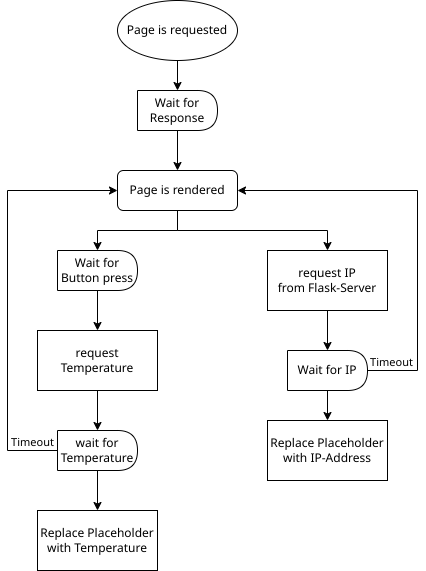
\includegraphics[width=0.7\textwidth]{topics/flowcharts/PageRender.png}
        \caption{Rendering process of the web page}
        \label{fig:webServer}
    \end{figure}
